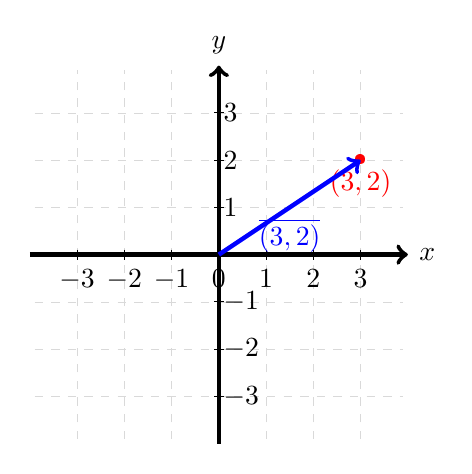
\begin{tikzpicture}[scale = 0.6]
\draw[help lines, color=gray!30, dashed] (-3.9,-3.9) grid (3.9,3.9);
\draw[->,ultra thick] (-4,0)--(4,0) node[right]{$x$};
\draw[->,ultra thick] (0,-4)--(0,4) node[above]{$y$};

\foreach \x in  {-3,-2,-1,0,1,2,3}
\draw[shift={(\x,0)},color=black] (0pt,3pt) -- (0pt,-3pt);
\foreach \x in {-3,-2,-1,0,1,2,3}
\draw[shift={(\x,0)},color=black] (0pt,0pt) -- (0pt,-3pt) node[below] 
     {$\x$};


\foreach \y in  {-3,-2,-1,1,2,3}
\draw[shift={(0, \y)},color=black] (3pt,0pt) -- (-3pt,-0pt);
\foreach \y in {-3,-2,-1,1,2,3}
\draw[shift={(0, \y)},color=black] (0pt,0pt) -- (-3pt,0pt) node[right] 
     {$\y$};
     

     \draw[red] (3,2) node[ultra thick]{\textbullet} node[below]{$(3,2)$};
     \draw[blue, ->, ultra thick] (0,0) -- (3,2) node[midway, below]{$\overline{(3,2)}$};

\end{tikzpicture}
